\chapter{Capacidad de las métricas}\label{sec:diferencias}
\addcontentsline{toc}{chapter}{Capacidad de las métricas}

En este capítulo se estudiará la capacidad de cada una de las métricas para realizar distinciones entre los grupos de alumnos en riesgo y los que no lo están.

\section{Estudio de las medidas de rendimiento clásicas}

\section{Estudio de las medidas de complejidad de propósito general}

\begin{figure}[H]
\centering
\subfloat[]{\label{fig:cl}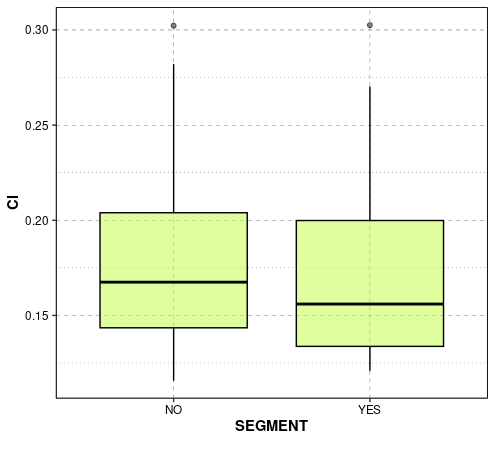
\includegraphics[width=0.46\textwidth]{diferencias/cl.png}}
\subfloat[]{\label{fig:de}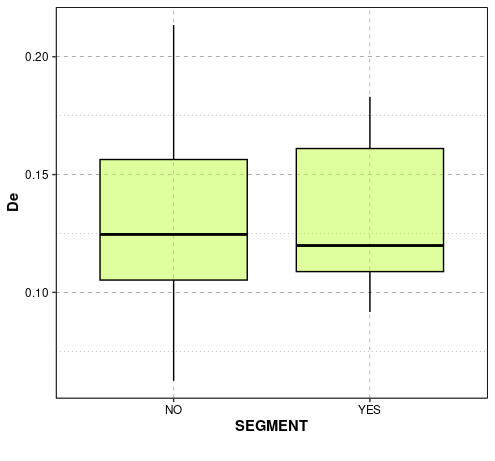
\includegraphics[width=0.46\textwidth]{diferencias/de.png}}
\subfloat[]{\label{fig:dm}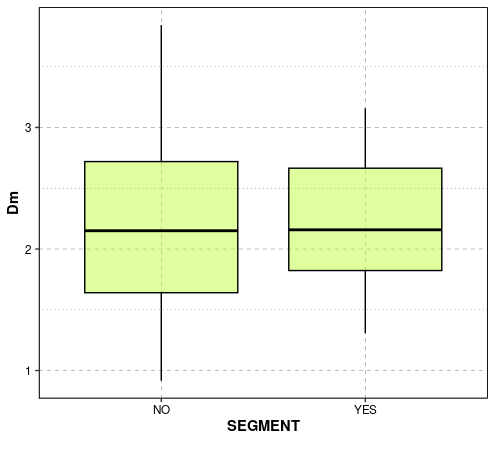
\includegraphics[width=0.46\textwidth]{diferencias/dm.png}}
\subfloat[]{\label{fig:le}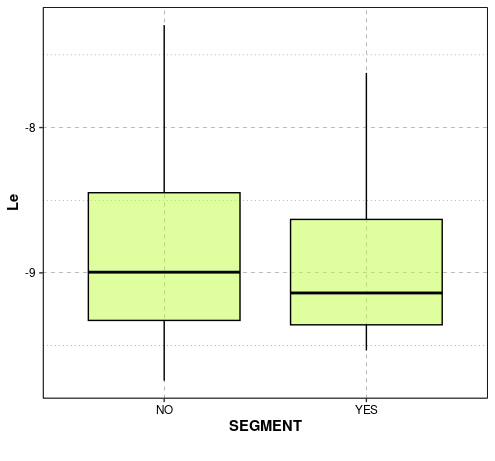
\includegraphics[width=0.46\textwidth]{diferencias/le.png}}
\subfloat[]{\label{fig:di}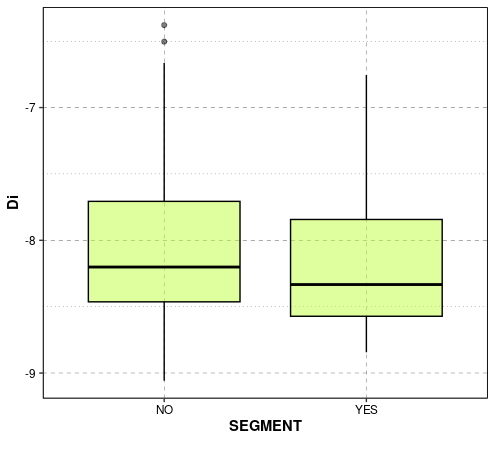
\includegraphics[width=0.46\textwidth]{diferencias/di.png}}
\subfloat[]{\label{fig:we}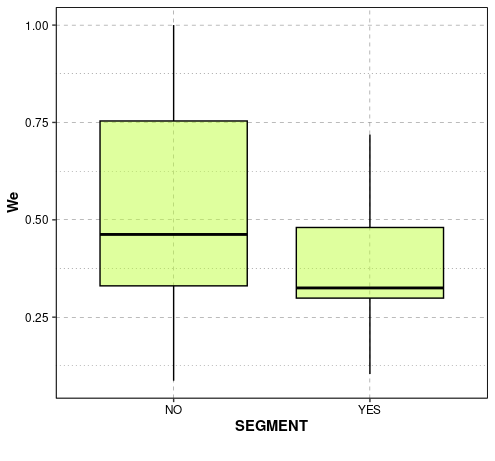
\includegraphics[width=0.46\textwidth]{diferencias/we.png}}
\subfloat[]{\label{fig:ef}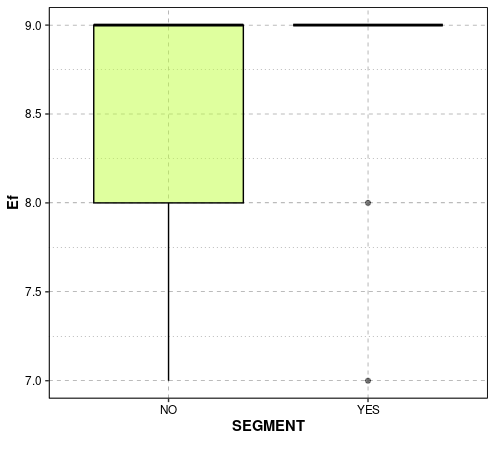
\includegraphics[width=0.46\textwidth]{diferencias/ef.png}}
\subfloat[]{\label{fig:st}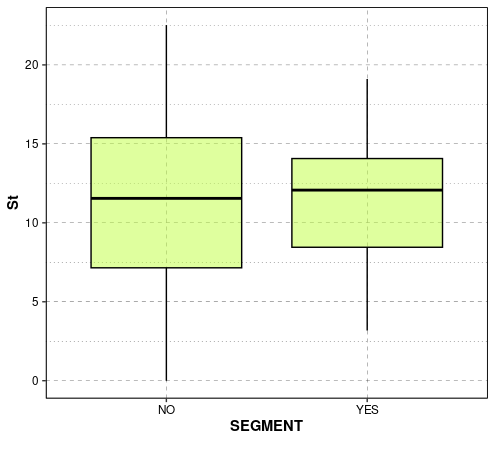
\includegraphics[width=0.46\textwidth]{diferencias/st.png}}
\subfloat[]{\label{fig:dag}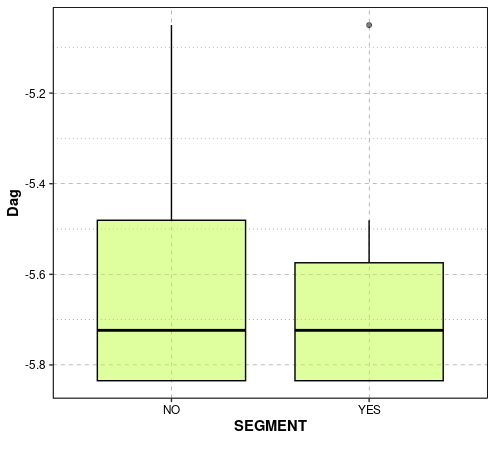
\includegraphics[width=0.46\textwidth]{diferencias/dag.png}}
\subfloat[]{\label{fig:wdag}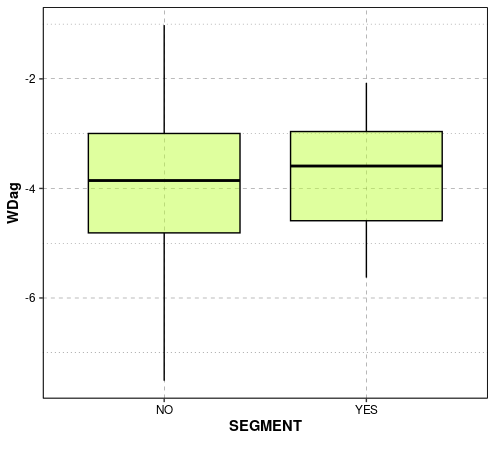
\includegraphics[width=0.46\textwidth]{diferencias/wdag.png}}
\subfloat[]{\label{fig:be}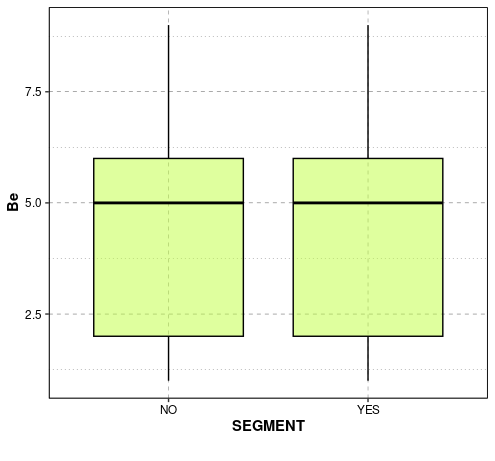
\includegraphics[width=0.46\textwidth]{diferencias/be.png}}
\subfloat[]{\label{fig:ba}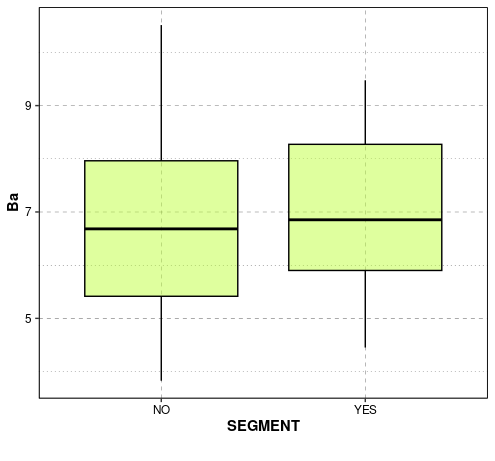
\includegraphics[width=0.46\textwidth]{diferencias/ba.png}}
\caption{Burdown charts de los seis primeros sprints del proyecto.}
\label{fig:separation}
\end{figure}
